\documentclass[tikz,12pt,border=3pt]{standalone}

% pdfcrop a2.pdf a2_crop.pdf; pdftocairo -singlefile -r 250 -png a2_crop.pdf a2;

\usepackage{pgfplots}
\usepackage{physics}
\usepackage{txfonts}
\usepgfplotslibrary{fillbetween}
\pgfplotsset{compat=1.12}
\usepackage{xcolor}

\definecolor{myred}{HTML}{cb181d}
\definecolor{myblue}{HTML}{2171b5}
\definecolor{mygreen}{HTML}{238b45}

\pgfmathsetmacro{\axl}{0.95}

% Glaciological convention (I don't agree with this); for Hills et al. review
\gdef\axnumA{1}
\gdef\axnumB{2}
\gdef\axnumC{3}
\gdef\isalt{-alt}

% PCA convention (first component is the first principal component)
%\gdef\axnumA{3}
%\gdef\axnumB{2}
%\gdef\axnumC{1}
%\gdef\isalt{}

%%%%%%%%%%%

\tikzset{
declare function={
	n00 = 0.28209479;
    fzis=-0.000000;fxis=0.000000;fyis=0.000000; gis=-0.000000; % iso
    fzsm=0.252313;fxsm=-0.126157;fysm=-0.126157; gsm=-0.000000; % SM symmetric
%    fzsx=0.252313;fxsx=-0.220774;fysx=-0.031539; gsx=-0.077255; % SM asymmetric
	fzgd=0.063078;fxgd=-0.126157;fygd=0.063078; ggd=-0.077255; % girdle
	%
	l1(\f,\g) = 1/3 + sqrt(2/15)* sqrt(2/3)*\f/n00;
	l2(\f,\g) = 1/3 + sqrt(2/15)* (-\g-1/2*sqrt(2/3)*\f)/n00;
	l3(\f,\g) = 1/3 + sqrt(2/15)* (+\g-1/2*sqrt(2/3)*\f)/n00;
	%
	Y00 = 1/sqrt(4*pi);
	Y20(\theta) = 1/4*sqrt(5/pi)*(3*cos(\theta)^2-1);
	%
	scale(\theta) = 3*sin(\theta);
	zz(\theta,\f) = scale(\theta)*( n00*Y00 + \f*Y20(\theta) ); 
	yy(\theta,\f) = scale(\theta)*( n00*Y00 + \f*Y20(\theta) ); 
	xx(\theta,\f) = scale(\theta)*( n00*Y00 + \f*Y20(\theta) ); 
}
}


\gdef\makepanel#1#2#3#4#5{
      
	\begin{axis}[
	    xshift=#5,
	    domain=+1:-1, no markers, view={90+40}{30}, axis line style=thick,
	    zmin=-1, zmax=1,  ymin=-1, ymax=1,  xmin=-1, xmax=1,
	    samples=100, samples y=0, axis lines=middle, % middle
	    xtick=\empty, ytick=\empty, ztick=\empty, 
	    xlabel=$\vb{m}_\axnumA$, xlabel style={below},
	    ylabel=$\vb{m}_\axnumB$, ylabel style={right},
	    zlabel=$\vb{m}_\axnumC$, zlabel style={above},
	    set layers,
	  ]
	
		\addplot3 [black, name path=Az] (0, x, 0);
		\addplot3 [black, name path=Bz] (x, 0, 0);
		\addplot3 [black, name path=Cz] (0, 0, x);
		
		\addplot3[mygreen, line width=1.25pt, name path=A] (0, x, {yy((1-x)*90,#2)});
		\addplot3[myblue,  line width=1.25pt, name path=B] (x, 0, {xx((1-x)*90,#3)});
		\addplot3[myred,   line width=1.25pt, name path=C] (0,    {zz((1-x)*90,#1)}, x);
				
		\addplot3[mygreen, opacity=0.25] fill between[of=A and Az];
		\addplot3[myblue,  opacity=0.25] fill between[of=B and Bz];
		\addplot3[myred,   opacity=0.25] fill between[of=C and Cz];
	
	\node[align=center,font=\fontsize{11.7}{12}\selectfont] (LBL) at (4.2em,4.2em) {
		$\textcolor{myred}{\lambdaup_\axnumC} = \pgfmathparse{l1(#1,#4)}\pgfmathprintnumber[precision=2]{\pgfmathresult}$\\[-0.em]
		$\textcolor{mygreen}{\lambdaup_\axnumB} = \pgfmathparse{l2(#1,#4)}\pgfmathprintnumber[precision=2]{\pgfmathresult}$\\[-0.em]
		$\textcolor{myblue}{\lambdaup_\axnumA} = \pgfmathparse{l3(#1,#4)}\pgfmathprintnumber[precision=2]{\pgfmathresult}$
	};	

	\end{axis}
}

\begin{document}

\gdef\figscale{0.77}
\gdef\DX{13em}
	
\begin{tikzpicture}[scale=1.0]
	
	\node[] at (45em,0) {\phantom{x}};

	\gdef\dxzero{8.0em}
	\gdef\dyzero{21em}
	
	\draw[-] (3.5em,14.25em) --++(36.5em,0) node[inner sep=0.75em,midway,fill=white] { ODFs projected onto principal directions $\vb{m}_i$};

	\node[] (ISO) at (0*\DX+\dxzero,\dyzero) {\includegraphics[scale=\figscale]{is-z\isalt.pdf}};	
	\node[yshift=0.6em] at (ISO.north) { \bf Isotropic};
	\makepanel{fzis}{fyis}{fxis}{gis}{0*\DX}

	\node[] (SM) at (1*\DX+\dxzero,\dyzero) {\includegraphics[scale=\figscale]{sm-z\isalt.pdf}};
	\node[yshift=0.6em] at (SM.north) { \bf Single maximum};
	\makepanel{fzsm}{fysm}{fxsm}{gsm}{1*\DX}

	\node[] (GD) at (2*\DX+\dxzero,\dyzero) {\includegraphics[scale=\figscale]{gd-z\isalt.pdf}};
	\node[yshift=0.6em] at (GD.north) { \bf Girdle};
	\makepanel{fzgd}{fygd}{fxgd}{ggd}{2*\DX}

	%%% EXPLAINING ARROWS

	\draw[->, very thick] (24.7em,2.5em) to[bend right] ++(-2em,1.8em) node[below,yshift=-1.5em,xshift=4em,align=center] {larger variance\\[-0.1em](larger eigenvalue)};

	\draw[->, very thick] (18.5em,2.6em) to[bend right] ++(0.5em,3em) node[below,yshift=-2.8em,xshift=-2em,align=center] {smaller variance\\[-0.1em](smaller eigenvalue)};
	
	%%% discrete c-axis distributions
	
%	\node[yshift=3em, xshift=2.5em] at (SM.east) {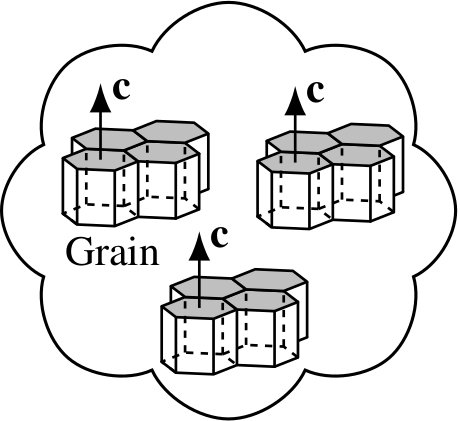
\includegraphics[scale=0.4]{/home/rathmann/Seafile/research/2020-specfab/images/tranisotropic/polycrystal-iceup.png}};

\end{tikzpicture}

\end{document}
